\section{Overzicht van het systeem}

\subsection{Het Systeem}

\begin{figure}[H]
	\centering
	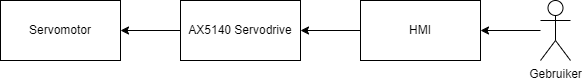
\includegraphics[width=\linewidth]{Systeemverband}
	\label{fig:SysteemVerband}
	\caption{Interfacing van gebruiker tot motor}
\end{figure}

In figuur \ref{fig:SysteemVerband} is de werking van het systeem te zien van de gebruiker tot de servomotor. De gebruiker kan via de \gls{HMI} de servodrive aansturen en daarmee dus ook de servomotor. De \gls{HMI} communiceert met de servodrive via \gls{EtherCAT} en \gls{SoE}. Standaard is dit \gls{EtherCAT} maar voor het schrijven en lezen van parameters gebruikt de drive \gls{SoE}.

\newpage

\subsection{Systeemcontext}

In figuur \ref{fig:Systeemcontext} is te zien waar de testkast gebruikt wordt. In eerste instantie wordt er een machine verkocht bij Voortman waar spindels in zitten voor het boren, tappen of vrezen van staal. Wanneer deze spindel na verloop van tijd niet meer correct functioneert wordt deze vervangen en wordt de kapotte spindel teruggestuurd richting Voortman. Hier wordt deze eventeel eerst getest als de oorzaak nog niet helemaal bekend is waarna de spindel gereviseerd wordt. Wanneer de spindel gereviseerd is zal deze nog getest worden om zeker te weten dat deze weer goed werkt waarna de spindel weer verkocht kan worden als gereviseerde spindel.

\begin{figure}[H]
	\centering
	\includegraphics[width=\linewidth]{Systeemcontext}
	\label{fig:Systeemcontext}
	\caption{Systeemcontext van de testkast}
\end{figure}

\newpage

\subsection{kritische analyse van de eisen}

In dit gedeelte van het functioneel ontwerp worden de belangrijkste eisen nog eens benoemd met daarbij de belangrijkste functies. Alle eisen staan gedefineerd in het SRD van de testkast (bijlage \ref{sec:TestKastSRD}).